
\newpage
\section{Evaluation}

Many people agree about the importance of designing systems for health and behaviour
change~\cite{article_mhealth, article_designing_for_healthy_lifestyles, article_designing_for_health_behaviour_change_hci}.
But each have varying opinions about how to evaluate these systems. Klasnja et al.~\cite{article_evaluate_tech_health_behaviour_change} focuses on system usability and does it meet the needs of users.
Whereas, Stawarz and Cox~\cite{article_designing_for_health_behaviour_change_hci} argue evaluating a system of this type requires information from other fields
to properly consider the systems effectiveness. The validated Behaviour Change Wheel Framework~\cite{article_behaviour_change_wheel} does just this.
Evaluating the system with validated behaviour change techniques from multiple domains. This project will use this framework to evaluate the chatbot with evaluation trials.
These will test the long-term effect and efficiency of the bot, with information from two fields of study, HCI and health psychology.

\subsection{Evaluation Trial Overview}
Evaluation trials are the final part of the Behaviour Change Wheel Framework~\cite{article_behaviour_change_wheel}.
HCI research that focuses on health interventions~\cite{article_mhealth}, demonstrates the importance of evaluation trials for evaluating mobile health systems.
These trials have three goals to test: objective-quantitative efficacy, subjective-qualitative feedback measures and real-world feedback about how the system is
utilised~\cite{article_evaluate_tech_health_behaviour_change}. I will conduct an evaluation trial for this project.\newline
\newline
The length of the trial will be based on two factors, the time needed to form a habit~\cite{article_how_habits_formed_modelling_habit_formation} and the results of a previous
habit formation trial~\cite{article_beyond_self_tracking_designing_apps}.
First, the number of repetitive days required for an action to be considered a habit varies based on the complexity of the action~\cite{article_how_habits_formed_modelling_habit_formation}.
Simple actions, such as drinking 2 glasses of water a day, can take a minimum of 18 days to form.
The suggested actions used for this project will be considered as simple, e.g. stretching for 30 seconds.
Second, a previous evaluation trial on habit-formation systems~\cite{article_how_habits_formed_modelling_habit_formation} showed an increase in habit automaticity after 4 weeks.
This project will mirror that timeframe.\newline
\newline
A 4-week evaluation trial will test the success of the chatbot by evaluating the tool and the effectiveness of each modality on users habit strength.
Chatbot interaction will be removed during the follow up study to test if users continue with the habit.
Participants will split into four groups, all groups will receive reminders, three groups will receive rewards each from a different modality,
and one group (control group) will not recieve any rewards.

\subsection{Testing Habit Strength}
Habit strength will be measured using a validated 12-question questionnaire that specifically looks at automaticity~\cite{article_habit_strength}.
Automaticity will also be measured using a validated subset of the questionnaire from~\cite{article_habit_strength} to test users habit behavioural
automaticity index~\cite{article_habit_measurement}. This will show the impact each modality has on habit automaticity and test the hypothesis.
Participants will fill out the questionnaires~\cite{article_habit_strength, article_habit_measurement} at three stages: half-way through the trial (at 2-weeks),
after the trial has finished and after the follow up trial.

\subsection{3-Week Trial}

Discussion of what a participant would actually do in this 3-week trail.\newline
Bullet point list based on beyond self tracking paper\newline
Ethics approval, Kathys PHD 5.3.\newline
How participants were recruited, screenshots of all adverts\newline
Creating the adverts\newline
Photo of website\newline
Photo of Screens users would see, facebook post, website, get started, Setup (Link to full setup screens in appendix), recieving reminder message, reward, snoozed lots messages, end of study messages.\newline


\subsection{1-Week follow up trial}

Discussion of what the expected behaviour of the participant should be, bullet point list.\newline
Transcript/screenshot of end of study messages.\newline
Talk about asking for interview.

\subsection{Interview}

General overview of interview questions.\newline
Informal chat.\newline
Questions:
  - General questions firsts
  - Habit formation insight
  - Chabot interaction
  - Modality interaction
  - Are you still doing that habit?
  - Why did you pick that habit?
  - Do you want it back?


\section{Results}

General discussion about how the results were analysed. Technology used. Security.\newline
'Does giving users too much personalisation effect the study?'\newline


\subsection{General Discussion}
General results analysed, with discussion. Lots of charts and graphs.

- Feedback
  - Add a 'before' or 'after' option to avoid sythetic awkwardness (erasmo)
  - Liked music rewards.
  - If you tell the bot they haven't done their habit after their context, when they snooze it isnt going to be their context anymore!!! e.g. lunch at 5pm. The solution is to remove habit context from snoozed reminders\newline

\subsubsection*{OLD STATS}
- 58 Unique users\newline
  - 19: iOS\newline
  - 13: Mac\newline
  - 13: Android\newline
  - 7: Windows\newline
  - 5: Linux\newline
- 5.4k total messages sent and recieved by the bot\newline
- Average >100 messages sent/received per each user\newline
- 55 users pressed got started (3 users didn't press get started)\newline
- 38 people completed their setup (17 People failed to setup)\newline
- 63\%/24 Male, 32\%/12 Female, 2 didnt say\newline
- More people snoozed EARLY\_MORNING (16), MID\_MORNING (38 snooze presses),\newline LATE\_AFTERNOON (14) and LATE\_EVENING (17 snooze presses)
- Most people chose Meditation as their habit (12 people), followed up Press ups (9) and\newline stretching (8)
- Average age was 26.6 (3 outliers of 57, 63 and 53. Removing these gives us 23 avg)\newline
- Only 7 people have used habit apps before\newline
- Most people set a reminder time for the evening (21), most LATE\_EVENING (10)\newline
- Most people snoozed PRESS\_UPS (49), MEDITATION (41) and STRETCH (22)\newline
- Users combined streaks were higher for MEDITATION and PRESS\_UPS (both 18 total)\newline
- Highest streak was 10 (stretching)\newline
- 18 daily active users :/\newline
- Talk about male female split\newline

\subsection{Key results}

Key questions answered, with discussion about what the key questions mean.\newline

\large{Was the chatbot successful at running a trial?}\newline
\large{Did users habit automaticity increase after using the chatbot?}\newline
\large{Did users habit automaticity increase when using a specific reward?}


\subsection{Issues}
Issues with study results and general issues with implementation.

Discussion about the issues I had w the bot
\begin{figure}[H]
  \centering
  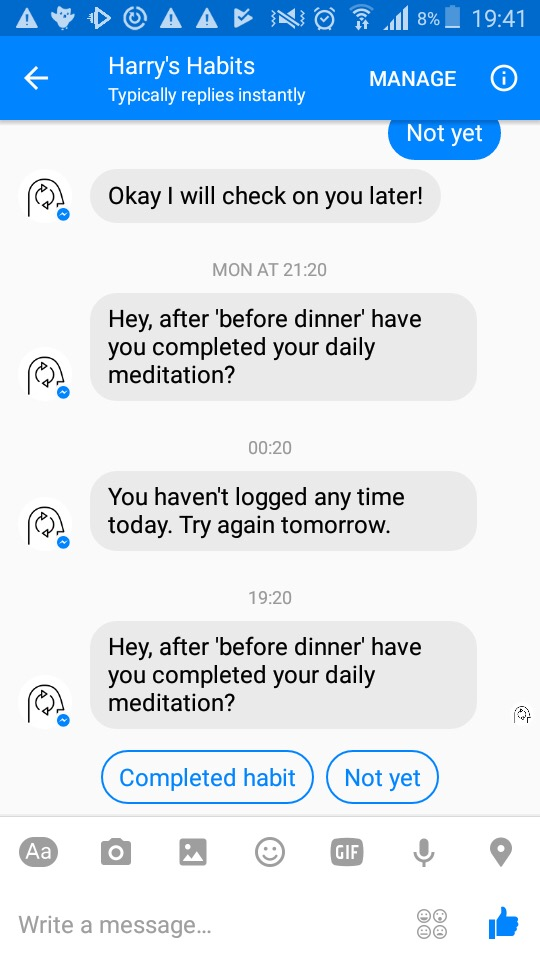
\includegraphics[width=2.1in]{../resources/feedback/after-before.jpg}
  \hspace{10px}
  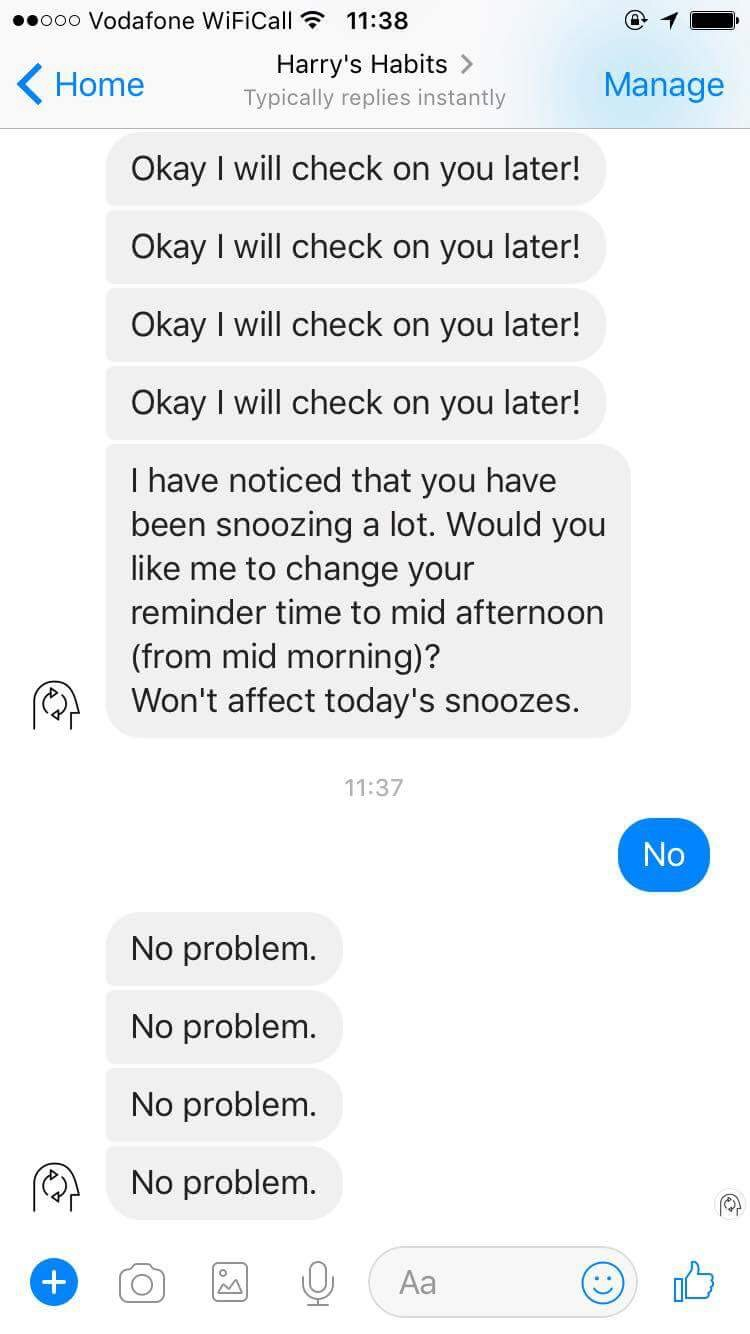
\includegraphics[width=2.1in]{../resources/feedback/double-messages.jpg}
  \caption{Example of 2 issues that occured, habit context using the word `after' and the bot sending multiple of the same messages.}
  \label{fig:study_bot_issues}
\end{figure}



\subsection{Summary}

Are the results even valid? What did we find out about the trail? Did we answer our research question?


